%Frequently update this section from aja/docs/latex_tutorial/latex_template.tex
%To get all latest inclusion updates on book seetings.

%TODO: This should be made as book template for aja use!
%memoir  is the book template from LaTeX
\documentclass[12pt, right open]{memoir}
%To draw stuff on out documents
\usepackage{graphicx}
\usepackage{tikz}
\usepackage{xcolor}
%indivudual library needed on ad-hoc basis
\usetikzlibrary{matrix,chains,positioning,decorations.pathreplacing,arrows,automata}
%To perform coordinate calculations, the calc library is required,
%calculations are enclosed in $
\usetikzlibrary{shapes.geometric, calc, intersections}
\usepackage{pgfplots}
%Maths tools
\usepackage{mathtools}
\usepackage{amsmath}
\usepackage{float}
\floatstyle{boxed}
\restylefloat{figure}
\usepackage{multirow} %for tables
\usepackage{ifthen}
%http://en.wikibooks.org/wiki/LaTeX/Algorithms
\usepackage{algorithmic}
\setcounter{secnumdepth}{5}

%To reduce vetical line spaces between list items
\usepackage{enumitem}
\setlist{nolistsep,leftmargin=*}

\newcommand{\specialcell}[2][c]{%
  \begin{tabular}[#1]{@{}c@{}}#2\end{tabular}}
%  Foo bar & \specialcell{Foo\\bar} & Foo bar \\    % vertically centered
%Foo bar & \specialcell[t]{Foo\\bar} & Foo bar \\ % aligned with top rule
%Foo bar & \specialcell[b]{Foo\\bar} & Foo bar \\ % aligned with bottom rule

%to tackle spaces in -1 n +1
\newcommand{\matplus}{
~~
  }

%For listing code
\usepackage{listings}
\usepackage{xcolor} % for setting colors

% set the default code style
\lstset{
    frame=tb, % draw a frame at the top and bottom of the code block
    tabsize=4, % tab space width
    showstringspaces=false, % don't mark spaces in strings
 %   numbers=left, % display line numbers on the left
    commentstyle=\color{green}, % comment color
    keywordstyle=\color{blue}, % keyword color
    stringstyle=\color{red} % string color
    breaklines=true,
}

\lstdefinestyle{codeTex}{
  belowcaptionskip=1\baselineskip,
  breaklines=true,
  frame=L,
  xleftmargin=\parindent,
  language=Tex,
  showstringspaces=false,
  basicstyle=\footnotesize\ttfamily,
  keywordstyle=\bfseries\color{green!40!black},
  commentstyle=\itshape\color{purple!40!black},
  identifierstyle=\color{blue},
  stringstyle=\color{orange},
}

\lstdefinestyle{codeC}{
  belowcaptionskip=1\baselineskip,
  breaklines=true,
  frame=L,
  xleftmargin=\parindent,
  language=C,
  showstringspaces=false,
  basicstyle=\footnotesize\ttfamily,
  keywordstyle=\bfseries\color{green!40!black},
  commentstyle=\itshape\color{purple!40!black},
  identifierstyle=\color{blue},
  stringstyle=\color{orange},
}
%\begin{lstlisting}[style=codeC]
%---------------
%\end{lstlisting}
%\lstinputlisting[caption=Scheduler, style=customc]{hello.c}


\begin{document}

%http://www.comp.leeds.ac.uk/ai23/reading/Hopfield.pdf

%TODO: Needs to find an easy way to draw neural nets

% >>>>>>>> Tikz Style sheet
% Create Tikz style, something like typedef in C, where we can specify the shape, color, size, text details etc

\tikzstyle{every pin edge}=[<-,shorten <=1pt]
\tikzstyle{neuron}=[circle,fill=black!10,minimum size=25pt,inner sep=0pt]
\tikzstyle{input neuron}=[neuron, fill=black!40]
\tikzstyle{output neuron}=[neuron, fill=black!40]
\tikzstyle{hidden neuron}=[neuron, fill=black!10]
\tikzstyle{annot} = [text width=4em, text centered]

\tikzstyle{startstop} = [rectangle, rounded corners, minimum width=3cm, minimum height=1cm,text centered, draw=black, fill=red!30]
\tikzstyle{io} = [trapezium, trapezium left angle=70, trapezium right angle=110, minimum width=3cm, minimum height=1cm, text centered, draw=black, fill=blue!30]
%\tikzstyle{process} = [rectangle, minimum width=3cm, minimum height=1cm, text centered, draw=black, fill=orange!30]
\tikzstyle{process} = [rectangle, minimum width=3cm, minimum height=1cm, text centered, text width=3cm, draw=black, fill=orange!30]
\tikzstyle{decision} = [diamond, minimum width=3cm, minimum height=1cm, text centered, draw=black, fill=green!30]
\tikzstyle{arrow} = [thick,->,>=stealth]
% <<<<<<<< Tikz Style sheet

\tableofcontents

%%%%%%%%%%%%%%%%%%%%%%%%%%%%%%%%%%%%%%%%%%%%%%%%%%%%%%%%%%%%%%%%%%%%%%%%%%%%%%%%%%%%%%%%%%%
\chapter{References for complex Latex commands}

\section{Maths}
% Use & to align the equation to the left marigin
\section{Weight Updation in Output Layer}
\begin{align*}
&W_{j,k} = W_{j,k}(t) + \Delta W_{j,k} \\
&\Delta W_{j,k} = \eta r x \\
&\text{In delta} \\
&r = (d_i - O_i) f' (O_{j,k})O_{j,k}
\end{align*}

%Sub heading in the chapter
\section{Basic Flowchart}

All flowcharts related latex commands can be followed here.
 
Reference: https://www.sharelatex.com/blog/2013/08/29/tikz-series-pt3.html

\begin{figure}[h!] %Create figure holder
\begin{tikzpicture}[node distance=2cm] %use the ‘tikzpicture’ environment

% Nodes are very powerful as we can easily position them, make them draw a shape, heavily format them and give them some text. In square brackets at the end of the begin command we specify a node distance of 2cm. This is so that the nodes we use to build the blocks are automatically spaced 2cm apart from their centres.

%      node_var  style   display text
\node (start) [startstop] {Start};
\node (in1) [io, below of=start] {Input};
\node (pro1) [process, below of=in1] {Process 1};
\node (dec1) [decision, below of=pro1] {Decision 1};
\node (dec1) [decision, below of=pro1, yshift=-0.5cm] {Decision 1};
\node (pro2a) [process, below of=dec1, yshift=-0.5cm] {Process 2a};
\node (pro2b) [process, right of=dec1, xshift=2cm] {Process 2b};
\node (out1) [io, below of=pro2a] {Output};
\node (stop) [startstop, below of=out1] {Stop};

\draw [arrow] (start) -- (in1);
\draw [arrow] (in1) -- (pro1);
\draw [arrow] (pro1) -- (dec1);
\draw [arrow] (dec1) -- (pro2a);
\draw [arrow] (dec1) -- (pro2b);
\draw [arrow] (dec1) -- node[anchor=east] {yes} (pro2a);
\draw [arrow] (dec1) -- node[anchor=south] {no} (pro2b);

\draw [arrow] (pro2b) |- (pro1);
\draw [arrow] (pro2a) -- (out1);
\draw [arrow] (out1) -- (stop);

\node (pro2a) [process, below of=dec1, yshift=-0.5cm] {Process 2a text text text text text text text text text text};

\end{tikzpicture}
\end{figure}

\begin{lstlisting}[style=codeTex]
% Create Tikz style, something like typedef in C, 
where we can specify the shape, color, size, text details etc

\tikzstyle{startstop} = [rectangle, rounded corners, minimum width=3cm, 
minimum height=1cm,text centered, draw=black, fill=red!30]
\tikzstyle{io} = [trapezium, trapezium left angle=70, trapezium right angle=110, minimum width=3cm, minimum height=1cm, text centered, draw=black, fill=blue!30]
%\tikzstyle{process} = [rectangle, minimum width=3cm, minimum height=1cm, text centered, draw=black, fill=orange!30]
\tikzstyle{process} = [rectangle, minimum width=3cm, minimum height=1cm, text centered, text width=3cm, draw=black, fill=orange!30]
\tikzstyle{decision} = [diamond, minimum width=3cm, minimum height=1cm, text centered, draw=black, fill=green!30]
\tikzstyle{arrow} = [thick,->,>=stealth]

\begin{figure}[h!] %Create figure holder
\begin{tikzpicture}[node distance=2cm] %use the ‘tikzpicture’ environment

% Nodes are very powerful as we can easily position them, make them draw a shape, heavily format them and give them some text. In square brackets at the end of the begin command we specify a node distance of 2cm. This is so that the nodes we use to build the blocks are automatically spaced 2cm apart from their centres.

%      node_var  style   display text
\node (start) [startstop] {Start};
\node (in1) [io, below of=start] {Input};
\node (pro1) [process, below of=in1] {Process 1};
\node (dec1) [decision, below of=pro1] {Decision 1};
\node (dec1) [decision, below of=pro1, yshift=-0.5cm] {Decision 1};
\node (pro2a) [process, below of=dec1, yshift=-0.5cm] {Process 2a};
\node (pro2b) [process, right of=dec1, xshift=2cm] {Process 2b};
\node (out1) [io, below of=pro2a] {Output};
\node (stop) [startstop, below of=out1] {Stop};

\draw [arrow] (start) -- (in1);
\draw [arrow] (in1) -- (pro1);
\draw [arrow] (pro1) -- (dec1);
\draw [arrow] (dec1) -- (pro2a);
\draw [arrow] (dec1) -- (pro2b);
\draw [arrow] (dec1) -- node[anchor=east] {yes} (pro2a);
\draw [arrow] (dec1) -- node[anchor=south] {no} (pro2b);

\draw [arrow] (pro2b) |- (pro1);
\draw [arrow] (pro2a) -- (out1);
\draw [arrow] (out1) -- (stop);

\node (pro2a) [process, below of=dec1, yshift=-0.5cm] {Process 2a text text text text text text text text text text};

\end{tikzpicture}
\end{figure}
\end{lstlisting}
%\lstinputlisting[caption=FlowChart, style=codeTex]{}

\section{Tikz}
A library to draw graphics in LaTeX.
We will cover the basics here, most of the stuff are explained in the code.
\begin{lstlisting}[style=codeTex]
 \draw[] - command draws what comes next. Takes options in []
\end{lstlisting}

\begin{figure}[h!]
\caption{Basics 1}
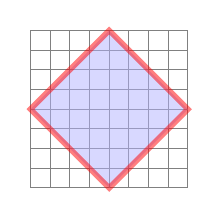
\begin{tikzpicture}
	\draw[step =0.25cm, color=gray]
	(-1,-1) grid (1,1);
	\draw[fill, color=blue!30, draw=red, 
			line width=2pt, opacity=0.5]
	(-1, 0) -- (0, 1) -- (1, 0) -- (0, -1) -- cycle;
\end{tikzpicture}
\end{figure}

\begin{figure}[h!]
\caption{Basics 2}
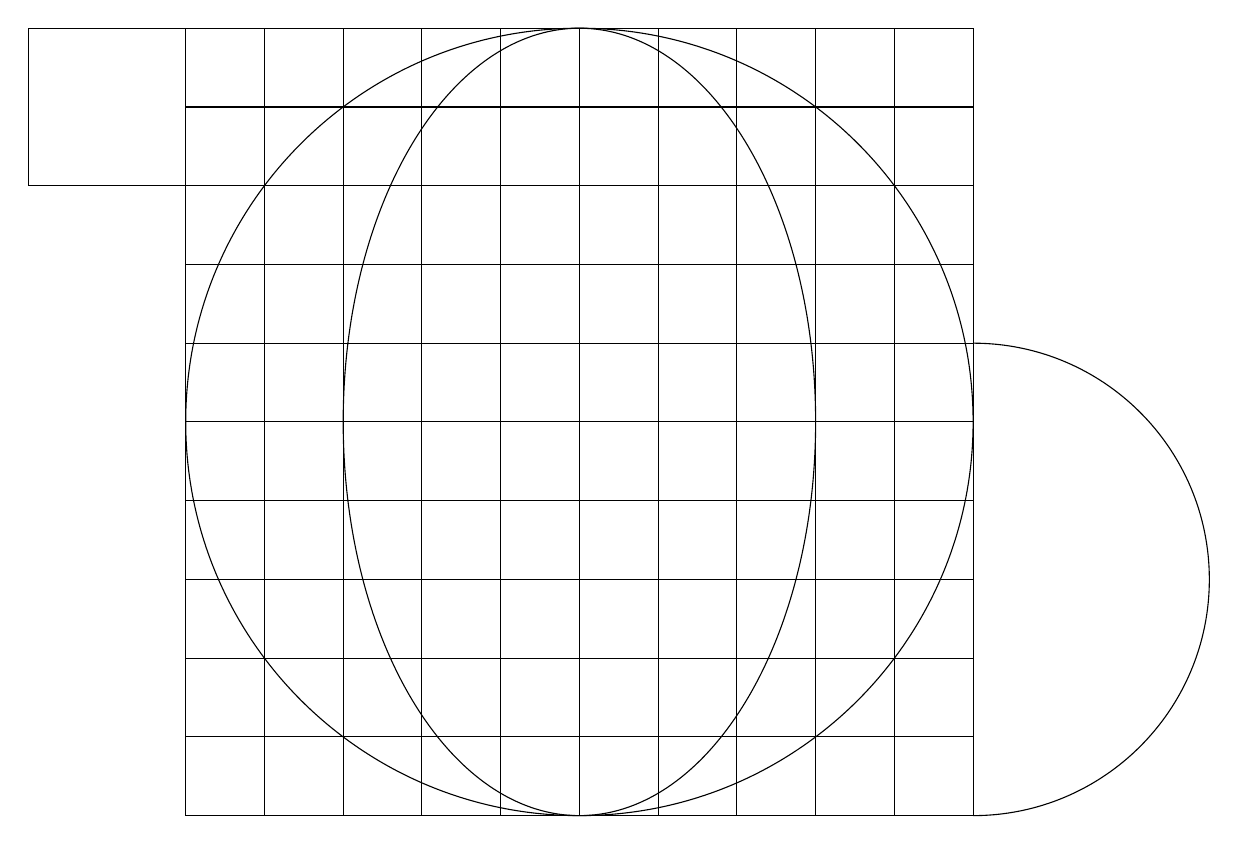
\begin{tikzpicture}
	\draw (0,0) grid (10,10);
	\draw (0,10) rectangle (-2,8);
	\draw (5,5) circle (5);
	\draw (5,5) circle(3 and 5);
	\draw (10,0) arc (-90:90:3); 
\end{tikzpicture}
\end{figure}

%Define the edges
\begin{figure}[h!]
\caption{Basics 3}
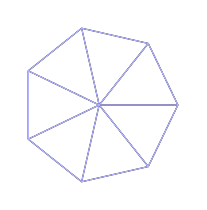
\begin{tikzpicture}

\coordinate (origin) at (0,0);
\coordinate (A) at (360.0 / 7.0 * 0 : 1);
\coordinate (B) at (360.0 / 7.0 * 1 : 1);
\coordinate (C) at (360.0 / 7.0 * 2 : 1);
\coordinate (D) at (360.0 / 7.0 * 3 : 1);
\coordinate (E) at (360.0 / 7.0 * 4 : 1);
\coordinate (F) at (360.0 / 7.0 * 5 : 1);
\coordinate (G) at (360.0 / 7.0 * 6 : 1);

%Draw the edges
\draw (A) -- (B) -- (C) -- (D) -- (E) -- (F) -- (G) -- cycle;

%Add spikes
\draw (origin) -- (A)
      (origin) -- (B)
      (origin) -- (C)
      (origin) -- (D)
      (origin) -- (E)
      (origin) -- (F)
      (origin) -- (G);
      
\foreach \i in {0,...,6}
{ 
	\draw [color= blue!30] (0,0) -- (360.0 / 7.0 * \i : 1)
								 -- ({360.0 / 7.0 * (\i + 1)}:1);
								 %{} - Indicates maths calculation
}
\end{tikzpicture}
\end{figure}

\begin{figure}[h!]
\caption{Basics 4}
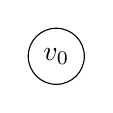
\begin{tikzpicture}
%\node [styke name] ...
\node (node_name) at (0,0) [draw,circle] {$v_0$};
\end{tikzpicture}
\end{figure}

\begin{figure}[h!]
\caption{Basics 5}
%To avoid typing it again and again
\tikzstyle{every node}=[draw, shape=circle]
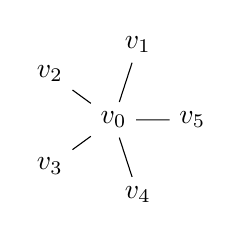
\begin{tikzpicture}
\node (v0) at (0,0) {$v_0$};
\node (v1) at (1*72:1) {$v_1$};
\node (v2) at (2*72:1) {$v_2$};
\node (v3) at (3*72:1) {$v_3$};
\node (v4) at (4*72:1) {$v_4$};
\node (v5) at (5*72:1) {$v_5$};

\draw (v0) -- (v1)
	  (v0) -- (v2)
	  (v0) -- (v3)
	  (v0) -- (v4)
	  (v0) -- (v5);

\end{tikzpicture}
\end{figure}

\begin{figure}[h!]
\caption{Basics 5}
%To avoid typing it again and again
\tikzstyle{every node}=[draw, shape=circle]
\begin{tikzpicture}
\coordinate[label=below:$A$] (A) at (2,1);
\fill (A) circle (2pt);
\fill[red] ($2*(A)$) circle (2pt);
\fill[green] ($(A) + (-1, 1)$) circle (2pt);
\fill[blue] ($(A) - (-1, 1)$) circle (2pt);
\end{tikzpicture}
\end{figure}

%\tikzstyle{probState}=[ circle,
%                    thick,
%                    minimum size=45pt,
%                    draw=blue!50,
%                    fill=white,
%                    line width=2.5pt,
%                    font=\large]
%\node [probState] (test){
%        \begin{tikzpicture}[trim axis left, trim axis right, baseline]
%        \begin{axis}[axis lines=none,width=80pt,height=80pt,
%         ylabel shift=-0.1cm]
%        \addplot[color=red]{1/(1+exp(-x))-2};
%        \end{axis}
%        \end{tikzpicture}
%    };
    
\begin{figure}[h!]
\caption{Basics 6}
    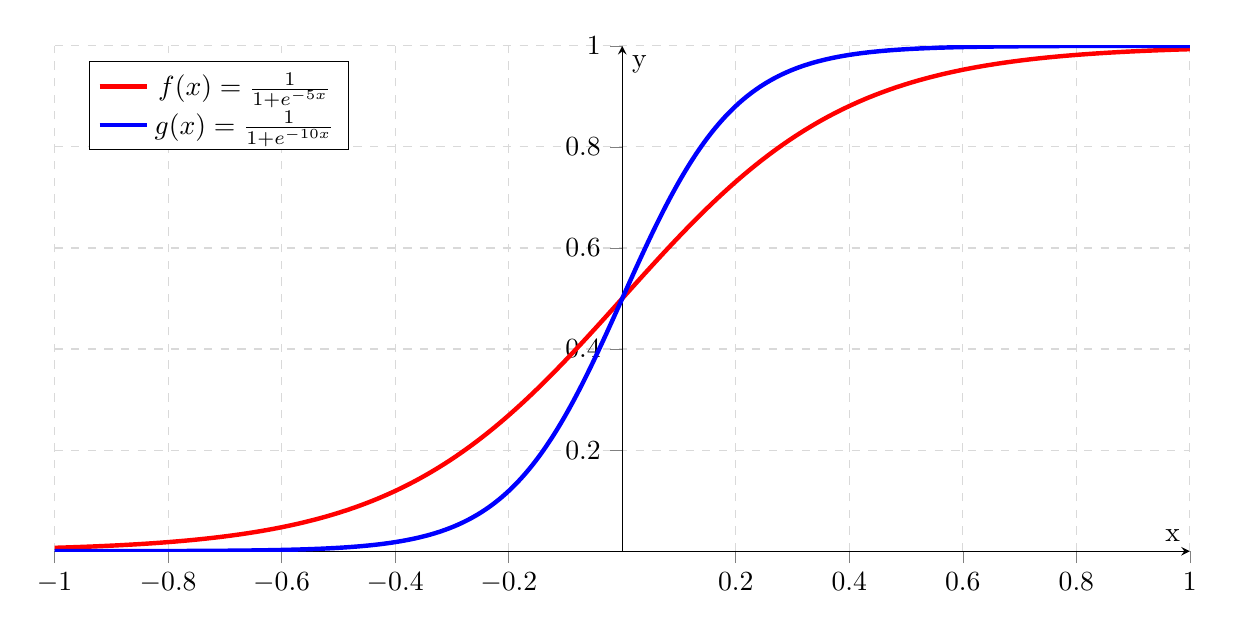
\begin{tikzpicture}
    \begin{axis}[
    	legend pos=north west,
        axis x line=middle,
        axis y line=middle,
        grid = major,
        width=16cm,
        height=8cm,
        grid style={dashed, gray!30},
        xmin=-1,     % start the diagram at this x-coordinate
        xmax= 1,    % end   the diagram at this x-coordinate
        ymin= 0,     % start the diagram at this y-coordinate
        ymax= 1,   % end   the diagram at this y-coordinate
        %axis background/.style={fill=white},
        xlabel=x,
        ylabel=y,
        tick align=outside,
        enlargelimits=false]
      % plot the stirling-formulae
      \addplot[domain=-1:1, red, ultra thick,samples=500] {1/(1+exp(-5*x))}; 
      \addplot[domain=-1:1, blue, ultra thick,samples=500] {1/(1+exp(-10*x))}; 
      \addlegendentry{$f(x)=\frac{1}{1+e^{-5x}}$}
      \addlegendentry{$g(x)=\frac{1}{1+e^{-10x}}$}
    \end{axis} 
\end{tikzpicture}
\end{figure}

\section{Neural Nets}
\def\layersep{2.5cm}
\begin{figure}[h!]
\caption{An artificial neuron as used in a Hopfield network} 
\label{fig:simple_neural_network}
\centering
\begin{tikzpicture}[shorten >=1pt,->,draw=black!50, node distance=\layersep]
    % Draw the input layer nodes
    \foreach \neuron in {1,...,3}
    % This is the same as writing \foreach \name / \y in {1/1,2/2,3/3,4/4}
    %Minus sign is to draw the neurons on top down fashion :P
        \node[input neuron] (I-\neuron) at (0,-\neuron) {\neuron};

    % Draw the output layer node
    \node[output neuron,pin={[pin edge={->}]right:Output}, right of=I-2] (Output) {o};

    % Connect every node in the input layer with the output layer
    \foreach \source in {1,...,3}
        \path (I-\source) edge node[above] {$w_\source$} (Output);

    % Annotate the layers
    \node[annot,below of=I-2] {Input layer};
    \node[annot,below of=Output] {Output layer};
\end{tikzpicture}
\end{figure}

\end{document}
